	
\section{Codificación de Voz}

Las redes de datos transfieren la información de modo digital y en VoIP la información que se maneja son señales de audio, principalmente señales de voz. Estas señales son analógicas por naturaleza, así que se requiere de un mecanismo que digitalice las señales analógicas, es decir, convierta las señales de voz en una secuencia de números discreta, para luego poder ser enviadas por la red y haga el proceso inverso al llegar a destino. 
Sí la solución VoIP implementada es completamente digital, éste proceso ocurre directamente en el teléfono (teléfonos digitales, celulares, micrófonos de computadores); en cambio, sí el sistema incluye secciones combinadas con telefonía tradicional, el proceso de digitalización ocurre en las intersecciones de los sistemas, bien sea en las pasarelas (gateways) del sistema o en conectores ATA (Analog Thelephone Adapter) como se muestra en las siguientes figuras
[FIGURA \ref{fig:pasarela}]  [FIGURA \ref{fig:ata}].

	\begin{figure}[h]
		
		%nombre de la imagen, sin extencion. "width=\textwidth" ancho igual al texto
		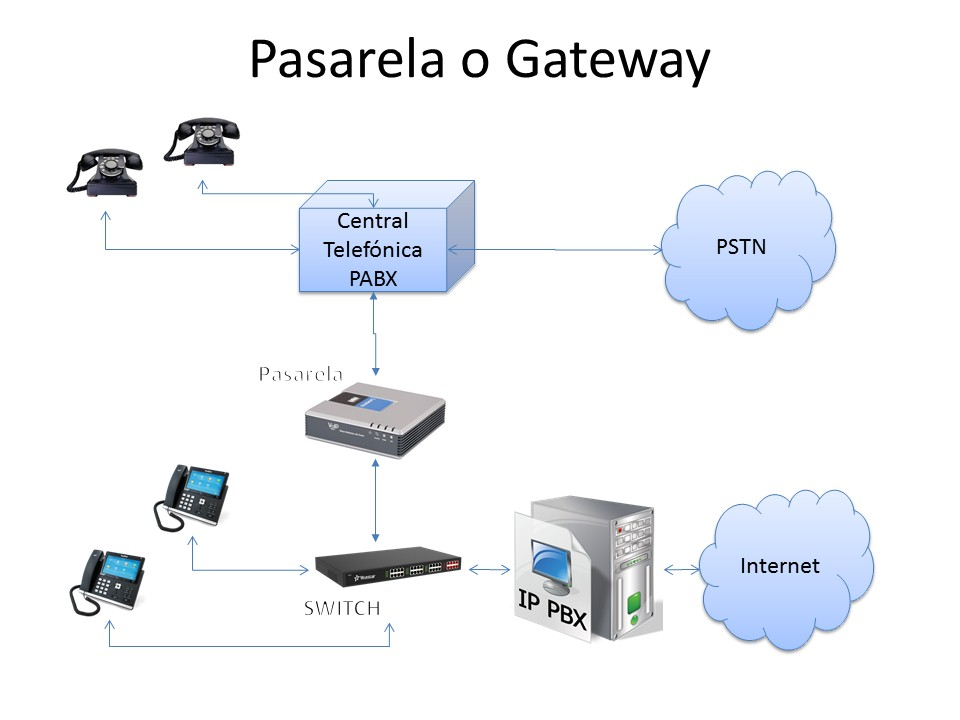
\includegraphics[scale=0.5]{pasarela}
		
		%titulo de la imagen, salen debajo de la imagen y en el indice de imagenes.
		\caption{VoIP combinada con telefonía tradicional a través de una pasarela}
		
		%centrado, por si las moscas
		\centering
		
		%para referencias
		\label{fig:pasarela}
	\end{figure}

Los primeros trabajos sobre digitalización de audio fueron realizados por el Ingeniero Alec Reeves poco antes de la segunda guerra mundial, quien desarrolló un sistema de audio digital con fines militares, sin embargo, la tecnología de comunicaciones de la época todavía no estaba lista para dicho avance. Alec Reeves patento un total de 82\footnote{http://www.quiantium.plus.com/ahr/patents.htm}  inventos entre los que se destaca la idea de Modulacion por impulsos codificados (PCM, Pulse Coded Modulation). Alrededor de los 60s fue que se popularizó la tecnología de PCM pero para entonces ya no eran reclamables los derechos de la patente.

	
		\begin{figure}[h]
			
			%nombre de la imagen, sin extencion. "width=\textwidth" ancho igual al texto
			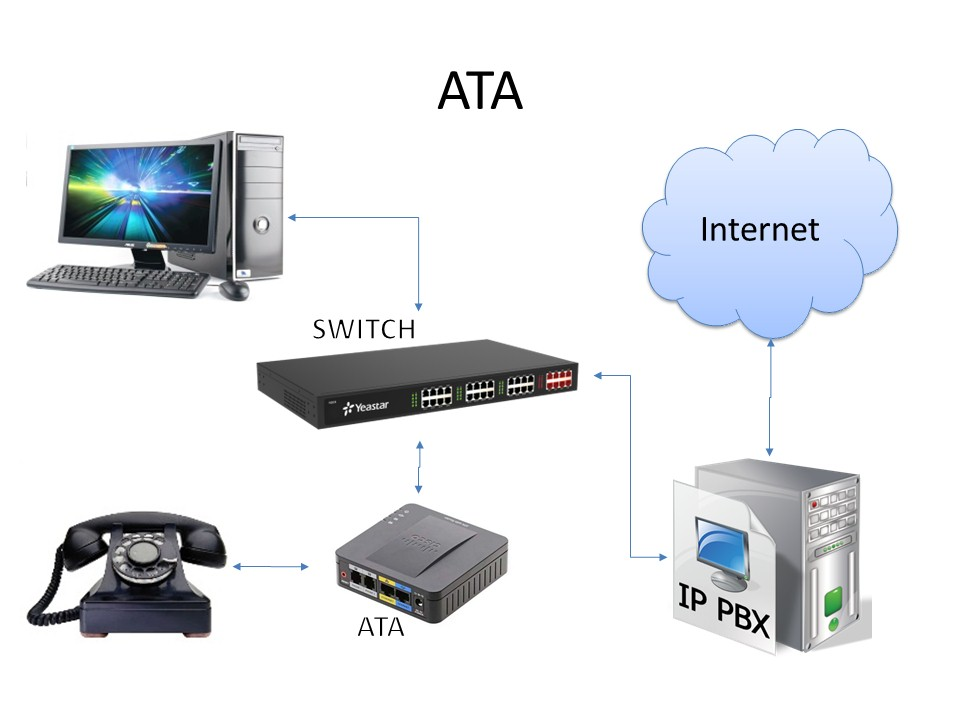
\includegraphics[width=\textwidth]{ata}
			
			%titulo de la imagen, salen debajo de la imagen y en el indice de imagenes.
			\caption{VoIP usando teléfonos analógicos y ATAs}
			
			%centrado, por si las moscas
			\centering
			
			%para referencias
			\label{fig:ata}
		\end{figure}
		
		
Inicialmente la digitalización de voz se basó en codificar la forma de onda de la señal analógica mediante un proceso de muestreo, cuantificación y codificación de la señal, el proceso de PCM. Luego, con el objetivo de reducir la tasa de bits requerida para transmitir la señal, se introdujeron las técnicas predictivas y comenzaron a codificar solo la diferencia entre los valores de las muestras reales y la predicción de la señal en base a la extrapolación de las muestras anteriores.

\subsection{Proceso de digitalización}



\subsection{Códec}

Los códec son algoritmos o dispositivos que realizan la codificación y decodificación de la señal de audio, con usados a menudo en videoconferencias y emisiones de medios de comunicación. La mayoría de los códec provoca pérdidas de información ya que están diseñados para minimizar el tamaño de los datos digitales. Existen códec sin pérdida (lossless) que mantienen la calidad más precisa del sonido, pero generan datos digitales muy grandes que en VoIP no son necesarios.

AQUI VA LA TABLA DE NARROWBAND


Existe gran variedad de códecs en el mercado actual y su clasificación puede depender de varios aspectos como la técnica que usan para codificar, el ancho de banda que se muestra o incluso la tasa de bits resultante. En las siguientes tablas se puede apreciar las principales diferencias entre los códec más comunes. En la primera [] se pueden apreciar los principales códec de banda angosta, diseñados para digitalizar audio en frecuencias entre 300Hz y 3,4kHz. En la segunda [] se comparan los códec de banda amplia que reproducen señales entre 50Hz y 7kHz. En la tercera [] se encuentran los códec de banda super amplia (frecuencias de 50Hz a 14kHz) y banda completa (frecuencias de 50 Hz a 20 kHz).

AQUI VA LA TABLA DE wideBAND

AQUI VA LA TABLA DE superwideBANDy fullband


\section{Codificación de Video}

	